% paper proposal for the Modelica 2017 Conference

%%% By default the modelica LaTeX class uses bibtex and natbib for refrences
\documentclass{resources/modelica}
%%% As alternative also for unicode and @online support
%%% use the more modern biber and biblatex instead
%\documentclass[backend=biber]{modelica}
%\addbibresource{example-paper.bib}
%\usepackage[utf8]{luainputenc} % utf8 input encoding that should work for both pdflatex and lualatex, but might not be available in every installation
\usepackage[utf8]{inputenc} % utf8 input encoding which should work with pdflatex, but not lualatex
\usepackage{cleveref}

\hypersetup{%
	pdftitle  = {Towards a Standard-Conform, Platform-Generic and Feature-Rich Modelica Device Drivers Library},
	pdfauthor = {Bernhard Thiele, Thomas Beutlich, Volker Waurich, Martin Sjölund,
	Tobias Bellmann}, pdfsubject = {12th International Modelica Conference 2017},
  pdfkeywords = {Modelica, embedded systems, real-time simulation},
	colorlinks,
	linkcolor=black,
	urlcolor=black,
	citecolor=black,
	pdfpagelayout = SinglePage,
	pdfcreator = pdflatex,
	pdfproducer = pdflatex}

\lstset{language = c,
       % basicstyle=\fontsize{9pt}{10.5pt}\selectfont,
       basicstyle=\fontsize{9pt}{10.5pt}\ttfamily,
       backgroundcolor = \color{white}}
\newcommand{\clang}[1]{\lstinline[language=c]|#1|}

\newcommand{\modelica}[1]{\lstinline[language=modelica]|#1|}
\newcommand{\BTHI}[1]{{\color{blue}{$\parallel_\textrm{BTHI}$#1$\parallel$}}}
\newcommand{\TBEU}[1]{{\color{orange}{$\parallel_\textrm{TBEU}$#1$\parallel$}}}
\newcommand{\VWAU}[1]{{\color{red}{$\parallel_\textrm{VWAU}$#1$\parallel$}}}
\newcommand{\MSJO}[1]{{\color{green}{$\parallel_\textrm{MSJO}$#1$\parallel$}}}
\newcommand{\TBEL}[1]{{\color{magenta}{$\parallel_\textrm{TBEL}$#1$\parallel$}}}

\crefformat{footnote}{#2\footnotemark[#1]#3}

% begin the document
\begin{document}
\thispagestyle{empty}

\title{Towards a Standard-Conform, Platform-Generic and Feature-Rich Modelica Device Drivers Library}
\author[1]{Bernhard Thiele}
\author[2]{Thomas Beutlich}
\author[3]{Volker Waurich}
\author[1]{Martin Sjölund}
\author[4]{Tobias Bellmann}
\affil[1]{PELAB, Linköping University, Sweden, {\small\texttt{\{bernhard.thiele,martin.sjoelund\}@liu.se}}}
\affil[2]{ESI ITI GmbH, Germany, {\small\texttt{thomas.beutlich@esi-group.com}}}
\affil[3]{Chair of Construction Machinery, TU Dresden, Germany, {\small\texttt{volker.waurich@tu-dresden.de}}}
\affil[4]{Institute of System Dynamics and Control, DLR, Germany, {\small\texttt{tobias.bellmann@dlr.de}}}

\date{} % <--- leave date empty
\maketitle\thispagestyle{empty} %% <-- you need this for the first page
\abstract{%
There are many cases where simulation applications need to interact with their
environment. Typical examples are Human-in-the-Loop (HITL) simulators (including
flight, driving, and marine training simulators), Hardware-in-the-Loop (HIL)
simulators, but also offline process simulators which cannot operate in a
completely self-contained manner and therefore need to be coupled to external
applications. Embedded control applications are another related area which
requires that applications interact with their environment. The
\emph{Modelica\_DeviceDrivers} library, which had its first release as
open-source library in 2012, tries to cater for such use cases. This paper
describes the library for the first time and reports about the numerous
challenges that the project experienced to meet its goal of supporting several
platforms and tools within a standard-conform, platform-generic, feature-rich,
and easy-to-use Modelica library.}

\noindent\emph{Keywords: HITL, HIL, real-time, embedded control applications,
external C}

\section{Introduction}
\BTHI{Bernhard, Tobias}\\

The most common usage of Modelica models is for offline simulation experiments.
However, in many cases simulations need to interact with their environment or
other software components.
Typical examples are Human-in-the-Loop (HITL) simulators (including flight,
driving, and marine training simulators), Hardware-in-the-Loop (HIL) simulators,
but also offline process simulators which cannot operate in a completely
self-contained manner and therefore need to be coupled to external applications.
Furthermore, Modelica can be used for developing (model-based) control
applications which also require interaction with their environment.

There are different approaches for enabling the above mentioned applications in
the context of Modelica. Several development environments offer tool chains for
real-time simulation and/or model-based development of embedded control
applications.
Some of these environments can be coupled with Modelica tools, by wrapping code
which is generated from Modelica tools into respective third-party tool-internal
representations which can be connected to hardware devices in the respective
development environment (\textit{e.g.}, Dymola\footnote{Dassault Systèmes,
\url{https://www.3ds.com}} via its DymolaBlock interface to the
MATLAB/Simulink\footnote{\label{tmw}The MathWorks, \url{https://mathworks.com}}
tool chain, OpenModelica\footnote{Open Source Modelica Consortium (OSMC),
\url{https://www.openmodelica.org}} via customized tool chains
\citep{Worschech2012}, SimulationX\footnote{SimulationX by ESI,
\url{https://www.simulationx.com}} via Code Export for Simulink/Simulink
Coder\cref{tmw} or HIL environments like dSPACE
DS1006\footnote{\label{dspace}dSPACE, \url{https://www.dspace.com}}, NI
VeriStand\footnote{National Instruments, \url{http://www.ni.com}} or ETAS
LABCAR\footnote{ETAS, \url{http://www.etas.com}} \citep{Blochwitz2009}).
Sometimes it may also be possible for a Modelica tool to generate Functional
Mock-up Units (FMUs) which can be imported into compatible development
environments, like the tool chain provided for the SCALEXIO\cref{dspace}
platform.

The \emph{Modelica\_DeviceDrivers} (MDD) library uses a different approach.
The MDD library provides access to external devices by utilizing Modelica's external
function interface for interfacing to the C API of various device drivers directly from Modelica
models (see Section~\ref{ModelicaDeviceDrivers}).

Historically, the origins of the MDD library can be traced back to the
\emph{ExternalDevices} library \citep{Bellmann2009}, an internal
DLR\footnote{Deutsches Zentrum für Luft- und Raumfahrt (DLR), German Aerospace
Center, \url{http://www.dlr.de}} Modelica library developed for the interactive
simulation and visualization of Modelica models. The \emph{ExternalDevices}
library already supported UDP and shared memory communication
as well as several input devices (keyboard, 3Dconnexion
SpaceMouse\footnote{3Dconnexion, \url{https://www.3dconnexion.com}}, and game
controller). Additionally, it featured a model-integrated real-time
visualization system, the foundation of the later \emph{DLR Visualization} library \citep{Hellerer2014}.

However, the \emph{ExternalDevices} library was limited to
Microsoft Windows and was developed to be used only with
the Dymola tool. In the further course of development it was decided to
split the \emph{ExternalDevices} library into the commercial DLR
Visualization library and an open-source cross-platform hardware interface
library, the \emph{Modelica\_DeviceDrivers} library.


% \BTHI{TODO: Bernhard, Tobias , \cite{Elmqvist2009}}


\section{Modelica\_DeviceDrivers}
\label{ModelicaDeviceDrivers}
\BTHI{TODO: Bernhard, Thomas, Volker}

The MDD library allows to access hardware devices from Modelica models.
This is achieved by using the Modelica external C interface to call the
appropriate C driver functions provided by the underlying operating system (see
Section~\ref{sec:CrossPlatformSupport}).

The library is organized in several layers as indicated in
Figure~\ref{fig:MDDLayeredArchitecture}. It
provides two high-level Drag \& Drop block interfaces. The first (\texttt{Blocks}) is
compatible to Modelica 3.2, using the traditional \modelica{when sample()}
element for periodically calling Modelica functions from the \textsf{Function Layer}. The second
(\texttt{ClockedBlocks}) uses the synchronous language elements extension
introduced in Modelica 3.3 and is compatible with the
\emph{Modelica\_Synchronous} library \citep{Otter2012}. Due to this support the MDD
library formally depends on the \emph{Modelica\_Synchronous} library, but in
practice the \emph{Modelica\_Synchronous} library (and tool support for the
synchronous language elements extension) is only required if one actually wants
to use the clocked block interface.
\begin{figure}[htb]
\begin{center}
  \includegraphics[width=\columnwidth]{figures/MDDLayeredArchitecture}
  \caption{MDD layered architecture.}
  \label{fig:MDDLayeredArchitecture}
\end{center}
\end{figure}

\subsection{Cross-Platform Support}
\label{sec:CrossPlatformSupport}

Currently Microsoft Windows and Linux are supported as main platforms, but recent
prototypical work also targets popular embedded systems boards directly (see
Section~\ref{sec:EmbeddedControl}).

When accessing hardware devices, a Modelica model or
application calls Modelica functions from the \textsf{Function Layer} (see
Figure~\ref{fig:MDDLayeredArchitecture}). These Modelica functions provide a
generic interface to the underlying \textsf{C-Code Layer} which is accessed by
Modelica's external function interface.
The platform differentiation is handled in the \textsf{C-Code Layer} which
uses preprocessor directives for conditional inclusion/exclusion of
platform-specific code (\mbox{\clang{#if}}, \mbox{\clang{#else}},
\mbox{\clang{#endif}}, etc.) similarly to the code fragment below.
\begin{lstlisting}[language=C]
#if defined(_MSC_VER) || defined(__CYGWIN__) || defined(__MINGW32__)
#include <windows.h>
/* Microsoft Windows specific code goes here */
#elif defined(__linux__)
#include <unistd.h>
/* Linux specific code goes here */
#else
#error "Modelica_DeviceDrivers: Unsupported compiler or platform"
#endif
\end{lstlisting}

\subsection{Extended Tool Support}
\label{sec:ExtendedToolSupport}

Initially, the library was developed using the Dymola tool. Later, considerable
development efforts have been spent for supporting the library also within
SimulationX and, very recently, also within OpenModelica. For achieving this, it
was necessary to change parts of the library (under the constraint of
maintaining backwards compatibility), and at the same time, to extend the
abilities of respective tools (partly by providing support for constructs which
are not (yet) allowed by the Modelica language standard).
This is discussed in more detail in Section~\ref{sec:ModelicaStandardCompliance}.


\subsection{Library Structure}
\label{sec:LibraryStructure}

Figure~\ref{fig:MDDPackageBrowseScreenshot} shows a screenshot of the package
browser view with loaded MDD library. The first two sub packages
\modelica{Blocks} and \modelica{ClockedBlocks} provide the drag \& drop blocks
which correspond to the \textsf{Block Layer} of
Figure~\ref{fig:MDDLayeredArchitecture}. The remaining sub packages (except
\modelica{Utilities} and \modelica{EmbeddedTargets}) provide the
\textsf{Function Layer}.
Both layers use sub packages for subdividing the provided functionality into
different groups. Package \modelica{EmbeddedTargets} contains highly
target specific function and blocks for supporting restricted
embedded systems like the Arduino microcontroller (see
Section~\ref{sec:Applications}).

\begin{figure}[htb]
  \centering
  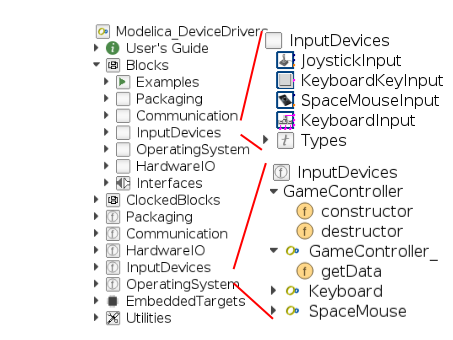
\includegraphics[width=\columnwidth]{figures/MDDPackageBrowseScreenshot}
  \caption{MDD library structure.}
  \label{fig:MDDPackageBrowseScreenshot}
\end{figure}

\BTHI{TODO continue}






\subsection{Interfaces}

\subsection{Features}

Features (aide-mémoire):
\begin{itemize}
  \item SerialPackager
  \item Communication
    \begin{itemize}
      \item UDP
      \item Shared Memory
      \item Softing CAN and Socket CAN
      \item RS232
    \end{itemize}
  \item input devices
    \begin{itemize}
      \item keyboard
      \item joystick/gamepad
      \item 3Dconnexion SpaceMouse
    \end{itemize}
  \item Operating System
    \begin{itemize}
      \item Realtime Synchronization
      \item Random numbers
    \end{itemize}
  \item Hardware I/O
    \begin{itemize}
      \item Comedi
    \end{itemize}
\end{itemize}


\noindent  New features:
\begin{itemize}
  \item Big endian
  \item Serial port on Win
  \item TCP/IP client
  \item LCM / UDP Broadcast
  \item Bluetooth
  \item MQTT
  \item \ldots
\end{itemize}

\section{Modelica Standard Compliance}
\label{sec:ModelicaStandardCompliance}
\BTHI{TODO: Thomas, Bernhard}

\subsection{Enhancements}

\subsection{Pitfalls and Open Issues}

Aide-mémoire:
\begin{itemize}
  \item Serialpackager
  \item Automatic buffer size
  \item External objects in equation
  \item Construction of external objects in record
  \item Linking to platform-dependent system libraries
  \item Missing fixed attribute for String
  \item Support of several include directories
\end{itemize}

\section{Applications}
\label{sec:Applications}

\subsection{Arduino}
\BTHI{TODO: Volker}

The Arduino\footnote{Arduino, \url{https://www.Arduino.cc}} is an open-source electronics platform which makes it very easy to read sensors, process the data and send it to another device via a serial connection.
With the help of the \emph{Modelica\_DeviceDrivers} serial port implementation, the Arduino can be utilized to make sensor data available in a real-time Modelica model.
Using different kinds of potentiometers, it is possible to build customized control devices.
As an exemplary application, pedals for a driving simulator can be equipped with a rotary potentiometer in order to measure the displacement.
This data can be send via a serial connection to a \textit{Blocks.Communication.SerialPortReceive} in order to drive a virtual vehicle.
Hence, expensive or unavailable input devices can be substituted by self-built constructions.
By using a Bluetooth module, a wireless connection between Arduino and the simulator is set up easily.
\VWAU{I could add Arduino code or an Arduino circuit diagram here.}

\subsection{Arduino, Raspberry PI, embedded control}
\label{sec:EmbeddedControl}
\BTHI{TODO: Bernhard, Martin}

\subsection{HID Joystick}
\BTHI{TODO: Volker }

\subsection{DLR Demonstrators}
\BTHI{TODO: Tobias}

\section{Outlook}
\BTHI{TODO: Bernhard, Thomas, Volker}

\section*{Acknowledgements}


%%% choose one of the following: %%%
%% References using bibtex (default)
\bibliography{modelica2017_Modelica_DeviceDrivers}

%% References using biber and biblatex
%\printbibliography

\end{document}
